%%%--------------------------------%%%
%%% UC10
%%%--------------------------------%%%

\newpage
% UC10 ====================================================
\subsubsection{Use Case Specification: \ac{UC}10 Activity Stream}
\label{sec:domainBbk}

\paragraph*{Description}\mbox{}\\
A user should be able to see the latest activities (see chapter \ref{sec:theoryBc}) in their project environment.

\paragraph*{Basic Flow} \mbox{}\\
\noindent
Activity Stream: 
\begin{itemize}
	\vspace{-3mm}
	\setlength\itemsep{-1em}
	\item The user opens the home page where the activity stream can be found.
	\item Within the activity stream the user can then find the latest activities .
	\item Depending on the activity the user has the chance to interact with the notification and will be redirected to the specific item (e.g. a user can click on a new risks shown in their activity stream to open it).
\end{itemize} 

\begin{figure}[H]
	\centering
	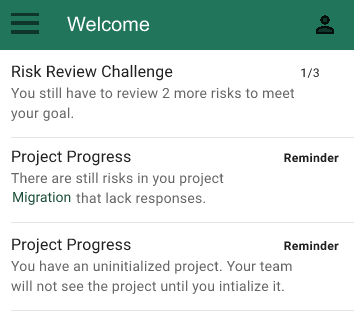
\includegraphics[width=0.5\textwidth]{Assets/UC_Screenshots/UC10S.png}
	\caption{Use Case 10: Mock Prototype}
	\label{fig:useCase10Detail}
\end{figure}

\paragraph*{Special Requirements and Preconditions}\mbox{}\\
As the activity contains personalized information, the following preconditions have to be fulfilled.
\begin{enumerate}
	\vspace{-3mm}
	\setlength\itemsep{-1em}
	\item The user has to be logged in.
	\item The user navigates to their personal home page.
\end{enumerate}
\newpage
\subparagraph{Activity Diagram}\mbox{}\\
\begin{figure}[H]
	\centering
	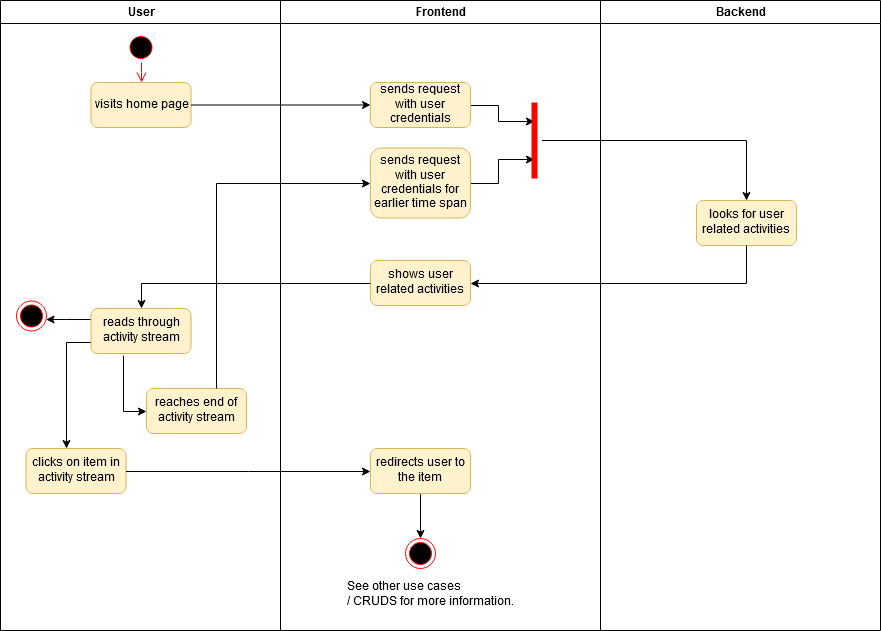
\includegraphics[width=0.9\textwidth]{Content/Domain/UC10ActivityStream.png}
	\caption{Activity Diagram \ac{UC}10 Activity Stream}
	\label{fig:label11}
\end{figure}

